% !TEX root = ./ECEN-629 - Homework 5 - Brody Jordan.tex

\documentclass[11pt]{article}

\usepackage[
    assignmentDueDate={December 1, 2025 at 11:00 am}
]{C:/Users/bljor/Sync/Courses/assignment}

\pgfplotsset{
    discard if not/.style 2 args={
        x filter/.code={
            \edef\tempa{\thisrow{#1}}
            \edef\tempb{#2}
            \ifx\tempa\tempb
            \else
                \def\pgfmathresult{NaN}
            \fi
        }
    }
}

\begin{document}
\makeAssignmentTitle


% ------ PROBLEM 1 ------ %
\begin{homeworkProblem}

    In many cases, we may need to compute the projection of a point onto a convex set (e.g.,
    in projected gradient descent). The projection of $x_0$ on convex set is defined as the optimal
    point for the following optimization problem:
    \begin{align*}
        \text{minimize:} \quad   & \norm{x - x_0}    \\
        \text{subject to:} \quad & x \in \mathcal{C}
    \end{align*}
    This projection is sometimes easy, sometimes hard. For the easy cases, analytical solutions
    can be found.
    \begin{enumerate}[label=(\alph*), topsep=5pt, itemsep=5pt]
        \item Suppose the norm we use is the $\ell_\infty$ norm, and the set $\mathcal{C}$ is $\{ x \mid \norm{x}_2 \leq 1 \}$.
              Find the projection of $x_0$.
        \item Suppose the norm we use is the $\ell_2$ norm, and the set $\mathcal{C}$ is $\{ x \mid \norm{x}_2 \leq 1 \}$.
              Find the projection of $x_0$.
        \item Suppose the norm we use is the $\ell_\infty$ norm, and the set $\mathcal{C}$ is $\{ x \mid l \preceq x \preceq u \}$.
              Find the projection of $x_0$.
        \item Suppose the norm we use is the $\ell_2$ norm, and the set $\mathcal{C}$ is $\{ x \mid l \preceq x \preceq u \}$.
              Find the projection of $x_0$.
        \item Suppose the norm we use is the $\ell_1$ norm, and the set $\mathcal{C}$ is $\{ x \mid l \preceq x \preceq u \}$.
              Find the projection of $x_0$.
        \item Suppose the norm we use is the $\ell_2$ norm, and the set $\mathcal{C}$ is $\{ x \mid Ax = b \}$. Find the projection
              of $x_0$. Assume the matrix $A$ has full row rank, and has more columns than rows.
        \item Provide one example of a convex set $\mathcal{C}$ that this projection is not easy to obtain analytical
              solutions or to compute. \newline
    \end{enumerate}
    \solution

    \textbf{Part (a):} Here
    \begin{align*}
        \text{minimize:} \quad   & \norm{x - x_0}_\infty \\
        \text{subject to:} \quad & \norm{x}_2 \leq 1
    \end{align*}
    \textbf{Part (b):} Here
    \begin{align*}
        \text{minimize:} \quad   & \norm{x - x_0}_2  \\
        \text{subject to:} \quad & \norm{x}_2 \leq 1
    \end{align*}
    \textbf{Part (c):} Here
    \begin{align*}
        \text{minimize:} \quad   & \norm{x - x_0}_\infty \\
        \text{subject to:} \quad & l \preceq x \preceq u
    \end{align*}
    \textbf{Part (d):} Here
    \begin{align*}
        \text{minimize:} \quad   & \norm{x - x_0}_2      \\
        \text{subject to:} \quad & l \preceq x \preceq u
    \end{align*}
    \textbf{Part (e):} Here
    \begin{align*}
        \text{minimize:} \quad   & \norm{x - x_0}_1      \\
        \text{subject to:} \quad & l \preceq x \preceq u
    \end{align*}
    \textbf{Part (f):} Here
    \begin{align*}
        \text{minimize:} \quad   & \norm{x - x_0}_2 \\
        \text{subject to:} \quad & Ax = b
    \end{align*}
    \textbf{Part (g):} In the case where $\mathcal{C}$ is an open set.

\end{homeworkProblem}

\pagebreak

% ------ PROBLEM 2 ------ %
\begin{homeworkProblem}

    Consider the problem:
    \begin{align*}
        \text{minimize:} \quad   & \text{length}(x)                \\
        \text{subject to:} \quad & \norm{Ax - b} \leq \varepsilon,
    \end{align*}
    where the length function $\text{length}(x) = \min\{ k \mid x_i = 0 \text{ for } i > k \} $. The decision variables $x \in \R[n]$, and
    $A$, $b$, and $\varepsilon$, are fixed parameters.
    \begin{enumerate}[label=(\alph*), topsep=5pt, itemsep=5pt]
        \item Show the problem is not convex;
        \item Show the problem is quasiconvex;
        \item Is the length function equivalent to the sparsity, i.e., the number of non-zero elements of $x$?
        \item (\textit{optional}) Formulate a problem where both the sparsity and the length of x are to be
              minimized. Proposal an approach to solve this problem efficiently. \newline
    \end{enumerate}
    \solution

    \textbf{Part (a):} Let $f(x) = \min\{ k \mid x_i = 0 \text{ for } i > k \} $. In order for this function to be convex, we require
    \[
        f(\theta x + (1 - \theta) y) \leq \theta f(x) + (1 - \theta) f(y)
    \]
    for all $x, y$ and $\theta \in [0, 1]$. That is not the case for this function, hence it is not convex. \\

    \textbf{Part (b):} In order for $f(x)$ to be convex, each sublevel set
    \[
        C_\alpha = \{ x \mid f(x) \leq \alpha \}
    \]
    must be convex for all $\alpha$. In this case, $C_\alpha = \{ x \mid \text{length}(x) \leq \alpha \}$. Which defines a convex set for all $\alpha$. Hence, this problem is quasiconvex. \\

    \textbf{Part (c):} No. This function does not count the number of non-zero elements of $x$, it only deals with the position of non-zero elements (via index).

\end{homeworkProblem}

\pagebreak

% ------ PROBLEM 3 ------ %
\begin{homeworkProblem}
    Suppose the measurement noise of a scalar quantity $x$ has the truncated Gaussian distribution
    with parameter $a > 0 > b$, such that the observed measurement $y$ is distributed according to
    the following distribution
    \[
        p_x(y)=\frac{1}{\Phi \sqrt{2 \pi \sigma^2}} \exp \left[-\frac{(y-x)^2}{2 \sigma^2}\right], \quad \text { for } b \leq y-x \leq a
    \]
    and $p_x(y)=0$ otherwise, where $\Phi$ is a constant, and $\sigma^2$ is a fixed and known value.
    \begin{enumerate}[label=(\alph*), topsep=5pt, itemsep=5pt]
        \item Write down an expression for $\Phi$.
        \item Write down the ML estimation problem, when we have $m$ iid scalar samples $\{y_i\}$, as an
              optimization problem; simplify it into a standard convex optimization form.
        \item Suppose $m = 8$, $(y_1, y_2, . . . , y_8) = (-1, 3,-6, 6, 5, 5, 8, 7)$, $\sigma^2 = 1$, and $a = 7$ and $b = -10$.
              What is the solution to your optimization problem? \newline
    \end{enumerate}
    \solution

    \textbf{Part (a):}
    \[
        \int_{b+x}^{a+x} \frac{1}{\Phi \sqrt{2 \pi \sigma^2}} \exp \left[-\frac{(y-x)^2}{2 \sigma^2}\right] dy = 1
    \]

    \textbf{Part (b):} For iid samples,
    \[
        l(x) = \sum_{i=1}^{m} \ln(1) - \ln(\Phi \sqrt{2 \pi \sigma^2}) - \frac{(y_i - x)^2}{2 \sigma^2}
    \]
    Which turns into
    \begin{align*}
        \text{minimize:} \quad   & - \sum_{i=1}^{m} (y_i - x)^2                  \\
        \text{subject to:} \quad & b \leq y_i - x \leq a, \quad i = 1, \ldots, m
    \end{align*}

    \textbf{Part (c):} Now $m = 8$, $(y_1, y_2, \dots, y_8) = (-1, 3,-6, 6, 5, 5, 8, 7)$, $\sigma^2 = 1$, and $a = 7$ and $b = -10$.

\end{homeworkProblem}

\pagebreak

% ------ PROBLEM 4 ------ %
\begin{homeworkProblem}

    Write a simple supporting vector machine program using Matlab/CVX/Python as follows:
    \begin{enumerate}[label=(\alph*), topsep=5pt, itemsep=5pt]
        \item Write a function to generate $n = 800$ random points in the dimensional space from the
              Gaussian mixture distribution
              \begin{align*}
                   & P\left(x \mid \mu_{1, x}, \mu_{1, y}, \sigma_{1, x}^2, \sigma_{1, y}^2, \pi_1, \mu_{2, x}, \mu_{2, y}, \sigma_{2, x}^2, \sigma_{2, y}^2, \pi_2\right)                                \\
                   & =\frac{\pi_1}{2 \pi \sigma_{1, x} \sigma_{1, y}} \exp \left(-\frac{\left(x-\mu_{1, x}\right)^2}{2 \sigma_{1, x}^2}-\frac{\left(y-\mu_{1, y}\right)^2}{2 \sigma_{1, y}^2}\right)      \\
                   & \quad+\frac{\pi_2}{2 \pi \sigma_{2, x} \sigma_{2, y}} \exp \left(-\frac{\left(x-\mu_{2, x}\right)^2}{2 \sigma_{2, x}^2}-\frac{\left(y-\mu_{2, y}\right)^2}{2 \sigma_{2, y}^2}\right)
              \end{align*}
              where $(\mu_{1, x}, \mu_{1, y})=(0,0)$, $(\mu_{2, x}, \mu_{2, y})=(2,1)$, $(\sigma_{1, x}^2, \sigma_{1, y}^2)=(1,0.5)$, $(\sigma_{2, x}^2, \sigma_{2, y}^2)= (\sqrt{2}, 2)$, $\pi_1=0.4$ and $\pi_2=0.6$.
              In other words, in this mixture Gaussian distribution, the modes are chosen at $(0.4, 0.6)$ probability. Draw the scatter plot of these points, and
              label each point using either a square or a cross, depending on which mode $(-1 \text{ or } 1)$ the data point was produced from.
        \item Write a program to call an optimization solver to solve the dual optimization problem,
              to find the support vector classifier using $600$ samples, and plot the classifier and on the
              scatter plot of these $600$ samples.
        \item Classify the remaining $200$ (holdout) points using the classifier you obtained from SVM;
              plot (in a new figure) the $200$ points and classifier result. What is the error rate?
        \item Complete the task in (b) and (c) using existing Python/Matlab functions or packages.
              Compare to the result you obtained. \newline
    \end{enumerate}
    \solution

    \textbf{Part (a):}
    \begin{figure}[hpbt!]
        \centering
        \begin{tikzpicture}
            \begin{axis}[
                    width=9cm,
                    height=7cm,
                    xlabel={$x$},
                    ylabel={$y$},
                    grid=major,
                    legend pos=north west,
                    % Define style for scatter points
                    scatter/classes={
                            -1={mark=square*, blue, mark size=2pt},
                            1={mark=x, red, mark size=3pt, line width=1pt}
                        }
                ]
                % Plot Class -1 (Squares)
                % We filter the data where the 'label' column equals -1
                \addplot[
                    scatter,
                    only marks,
                    scatter src=explicit symbolic,
                    discard if not={label}{-1}
                ] table [x=x, y=y, meta=label] {svm_data.dat};

                % Plot Class 1 (Crosses)
                % We filter the data where the 'label' column equals 1
                \addplot[
                    scatter,
                    only marks,
                    scatter src=explicit symbolic,
                    discard if not={label}{1}
                ] table [x=x, y=y, meta=label] {svm_data.dat};

            \end{axis}
        \end{tikzpicture}
    \end{figure}

\end{homeworkProblem}

\pagebreak



% ------ PROBLEM 5 ------ %
\begin{homeworkProblem}

    Let $\gamma > 1$. The function
    \[
        f(x_1, x_2) = \begin{dcases}
            \sqrt{x_1^2 + \gamma x_2^2}                   & |x_2| \leq x_1 ;    \\
            \frac{x_1 + \gamma |x_2|}{\sqrt{1 + \gamma} } & \text{ otherwise} .
        \end{dcases}
    \]
    is convex.
    \begin{enumerate}[label=(\alph*), topsep=5pt, itemsep=5pt]
        \item Plot the function and visually identify (approximately) its optimal solution;
        \item Let $\gamma = 100$. Let $x^{(k)} = (1, 5)$ be the point in the $k$-th iteration. Find the search
              direction of the gradient descent method.
        \item Again let $\gamma = 100$, and let $x^{(k)} = (1, 5)$ be the point in the $k$-th iteration. Find the
              search direction of the steepest descent method under the $\ell_1$ norm;
        \item Again let $\gamma = 100$, and let $x^{(k)} = (1, 5)$ be the point in the $k$-th iteration. With the
              gradient descent method and backtracking line search of parameters $(\alpha, \beta) = (0.45, 0.9)$,
              will the step size be determined in two iterations in the line search procedure?
        \item Applying the gradient descent algorithm on this function, with starting point $x^{(0)} =
                  (\gamma, 1)$ with an exact line search. It can be shown that the iterations for $x^{(k)}_1$ is
              \[
                  x_1^{(k)} = \gamma\left(\frac{\gamma - 1}{\gamma + 1}\right)^k .
              \]
              Find the value $x_2^{(k)}$ in that corresponding iteration. What does the algorithm converge to? Is it optimal? \newline
    \end{enumerate}
    \solution

    \begin{figure}[hbpt!]
        \centering
        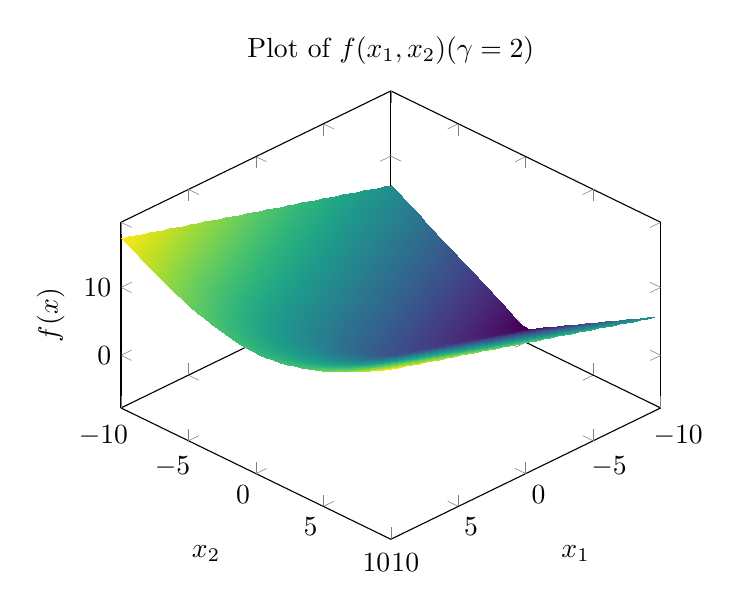
\begin{tikzpicture}
            \begin{axis}[
                    title={Plot of $f(x_1, x_2) (\gamma = 2)$},
                    xlabel={$x_1$},
                    ylabel={$x_2$},
                    zlabel={$f(x)$},
                    view={135}{45},
                    colormap/viridis,
                    domain=-10:10,
                    y domain=-10:10,
                    samples=40,
                    z buffer=sort,
                ]
                \def\gammav{2}

                \addplot3[
                    surf,
                    shader=interp,
                    z filter/.code={
                            \pgfmathparse{
                                (abs(y) <= x) ?
                                (sqrt(x^2 + \gammav * y^2)) :
                                ((x + \gammav * abs(y)) / sqrt(1 + \gammav))
                            }
                            \pgfmathresult
                        }
                ]
                {
                    (abs(y) <= x) * sqrt(x^2 + \gammav * y^2) +
                    (abs(y) > x) * ((x + \gammav * abs(y)) / sqrt(1 + \gammav))
                };

            \end{axis}
        \end{tikzpicture}
    \end{figure}


\end{homeworkProblem}

\pagebreak

% ------ PROBLEM 6 ------ %
\begin{homeworkProblem}

    Consider the optimization problem
    \begin{align*}
        \text{minimize:} \quad   & \log\left(\sum_{i=1}^{n} ie^{x_i}\right) + \sum_{i=1}^{n} i^2(x_i - i)^2 \\
        \text{subject to:} \quad & \sum_{i=1}^{n} x_i = P.
    \end{align*}
    \begin{enumerate}[label=(\alph*), topsep=5pt, itemsep=5pt]
        \item Let $P = 15$. Assume $n = 5$. If the starting point is $x^{(0)} = (1, 2, 3, 4, 5)$, find the gradient,
              the Hessian matrix, and the first Newton step. Write down the equation, but you can
              solve for it numerically.
        \item Let $P = 15$. Assume $n = 50$. Write you own Newton method program (in c/c++ or
              python) with infeasible start to calculate the optimal solution.
        \item Use CVX package to solve the same problem in (b). \newline
    \end{enumerate}
    \solution

    The gradient
    \[
        \nabla f = \frac{ie^{x_i}}{\sum_{j} je^{x_j}}  + 2i^2(x_i - i)
    \]
    The Hessian
    \[
        \nabla^2 f = \begin{bmatrix}
            \frac{e^{x_1}}{\sum_{k} ke^{x_k}} - \left(\frac{e^{x_1}}{\sum_{k} ke^{x_k}}\right)^2 + 2 & -\frac{1e^{x_2}1e^{x_2}}{\sum_{k} ke^{x_k}}                                                & -\frac{1e^{x_1}3e^{x_3}}{\sum_{k} ke^{x_k}}                                                 \\
            -\frac{2e^{x_2}1e^{x_1}}{\sum_{k} ke^{x_k}}                                              & \frac{4e^{x_2}}{\sum_{k} ke^{x_k}} - \left(\frac{2e^{x_2}}{\sum_{k} ke^{x_k}}\right)^2 + 8 & -\frac{2e^{x_2}3e^{x_3}}{\sum_{k} ke^{x_k}}                                                 \\
            -\frac{3e^{x_3}1e^{x_1}}{\sum_{k} ke^{x_k}}                                              & -\frac{3e^{x_3}2e^{x_2}}{\sum_{k} ke^{x_k}}                                                & \frac{9e^{x_3}}{\sum_{k} ke^{x_k}} - \left(\frac{3e^{x_3}}{\sum_{k} ke^{x_k}}\right)^2 + 18 \\
        \end{bmatrix}
    \]
    With $x_1 + x_2 + x_3 + x_4 + x_5 = 15$.

\end{homeworkProblem}

\pagebreak

% ------ PROBLEM 7 ------ %
\begin{homeworkProblem}

    Consider the optimization problem (similarly as above but with an inequality constraint)
    \begin{align*}
        \text{minimize:} \quad   & \log\left(\sum_{i=1}^{n} ie^{x_i}\right) + \sum_{i=1}^{n} i^2(x_i - i)^2 \\
        \text{subject to:} \quad & \sum_{i=1}^{n} x_i \leq P.
    \end{align*}
    \begin{enumerate}[label=(\alph*), topsep=5pt, itemsep=5pt]
        \item Let $P = 20$. Assume $n = 5$. If the starting point is $x^{(0)} = (1, 2, 3, 4, 5)$. Find the gradient
              and the Hessian of the logarithmic barrier function.
        \item Let $P = 20$. Assume $n = 5$. If the starting point is $x^{(0)} = (1, 2, 3, 4, 5)$. In the log barrier
              method (when $t = 10$), find the first Newton step. Write down the equation, but you
              can solve for it numerically.
        \item Use CVX package to solve the same problem in (b). \newline
    \end{enumerate}
    \solution

    The gradient
    \[
        \nabla f = \frac{ie^{x_i}}{\sum_{j} je^{x_j}}  + 2i^2(x_i - i)
    \]
    The Hessian
    \[
        \nabla^2 f = \begin{bmatrix}
            \frac{e^{x_1}}{\sum_{k} ke^{x_k}} - \left(\frac{e^{x_1}}{\sum_{k} ke^{x_k}}\right)^2 + 2 & -\frac{1e^{x_2}1e^{x_2}}{\sum_{k} ke^{x_k}}                                                & -\frac{1e^{x_1}3e^{x_3}}{\sum_{k} ke^{x_k}}                                                 \\
            -\frac{2e^{x_2}1e^{x_1}}{\sum_{k} ke^{x_k}}                                              & \frac{4e^{x_2}}{\sum_{k} ke^{x_k}} - \left(\frac{2e^{x_2}}{\sum_{k} ke^{x_k}}\right)^2 + 8 & -\frac{2e^{x_2}3e^{x_3}}{\sum_{k} ke^{x_k}}                                                 \\
            -\frac{3e^{x_3}1e^{x_1}}{\sum_{k} ke^{x_k}}                                              & -\frac{3e^{x_3}2e^{x_2}}{\sum_{k} ke^{x_k}}                                                & \frac{9e^{x_3}}{\sum_{k} ke^{x_k}} - \left(\frac{3e^{x_3}}{\sum_{k} ke^{x_k}}\right)^2 + 18 \\
        \end{bmatrix}
    \]
    With $x_1 + x_2 + x_3 + x_4 + x_5 \leq 15$.

\end{homeworkProblem}

\pagebreak

% ------ PROBLEM 8 ------ %
\begin{homeworkProblem}

    Consider the unconstrained optimization problem
    \begin{align*}
        \text{minimize:} \quad e^{x_1 + 2x_2} + x_2^2 + x_3^2 - x_2 x_3
    \end{align*}
    where $x = (x_1, x_2, x_3)^T \in \mathbb{R}^3$ is the variable. Let $x^{(k)} = (1, 1, 1)$ be the point in the $k$-th
    iteration.
    \begin{enumerate}[label=(\alph*), topsep=5pt, itemsep=5pt]
        \item Compute the next Newton step.
        \item Suppose the optimization problem has two additional constraints:
              \begin{align*}
                  x_1 + x_2 + x_3 & \leq 4  \\
                  x_2 - x_3       & \leq 2.
              \end{align*}
              Compute the next Newton step using the log-barrier method with the same $x^{(k)}$ and the
              barrier weighting parameter $t = 20$. \newline
    \end{enumerate}
    \solution

    \textbf{Part (a):} The Newton step
    \[
        \Delta x_\text{nt} = - \nabla^2 f(x)^{-1} \nabla f(x)
    \]
    with
    \[
        \nabla f(x) = \begin{bmatrix}
            e^{x_1 + 2x_2}               \\
            2e^{x_1 + 2x_2} + 2x_2 - x_3 \\
            x_2 + 2x_3                   \\
        \end{bmatrix}
    \]
    and
    \[
        \nabla^2 f(x) = \begin{bmatrix}
            e^{x_1 + 2x_2}  & 2e^{x_1 + 2x_2}     & 0  \\
            2e^{x_1 + 2x_2} & 2e^{x_1 + 2x_2} + 2 & -1 \\
            0               & 1                   & 2  \\
        \end{bmatrix}
    \] \\

    \textbf{Part (b):}

    \begin{align*}
        \text{minimize:} \quad   & e^{x_1 + 2x_2} + x_2^2 + x_3^2 - x_2 x_3 \\
        \text{subject to:} \quad & x_1 + x_2 + x_3 \leq 4                   \\
                                 & x_2 - x_3 \leq 2
    \end{align*}


\end{homeworkProblem}


\end{document}